\chapter{Manual de usuario}
\label{chap:manual}

El presente anexo se presenta un manual de usuario destinado a explicar todas las funcionalidades
desarrolladas del sistema desarrollado en este proyecto.

\section{Introducción}

El sistema consta de tres aplicaciones diferentes:

\begin{itemize}
  \item \textbf{Naviganto} Encargado de implementar todas las funciones de navegación por satélite y
    de comunicarse con los complementos vibratorios y activarlos.
  \item \textbf{Naviganto Bluetooth} Encargado de implementar el complemento vibratorio en
    Android.
  \item \textbf{Naviganto Wear} Encargado de implementar el complemento vibratorio en Android Wear.
\end{itemize}

Para el funcionamiento del sistema basta con instalar la aplicación \emph{Naviganto} en nuestro
dispositivo; pero sólo con esta aplicación no podremos hacer uso de la vibración para que nos guíe
en nuestra navegación. Por tanto, para el funcionamiento completo del sistema necesitaremos dos
dispositivos como mínimo: uno colocado en la parte izquierda de nuestro cuerpo y otro que
colocaremos en la parte derecha. En el cuadro~\ref{cuadro:convinacionesApps} se resumen todas las
posibles combinaciones válidas entre las aplicaciones del sistema para hacer uso del funcionamiento
completo.

\begin{table}[h]
  \centering
  \begin{tabular}{|l|l|l|}
    \hline
    \textbf{Naviganto} & \textbf{Naviganto Bluetooth} & \textbf{Naviganto Wear} \\
    \hline
    1 (izquierda) & 1 (derecha)             & 0                       \\
    \hline
    1 (derecha)   & 1 (izquierda)           & 0                       \\
    \hline
    1             & 2 (izquierda y derecha) & 0                       \\
    \hline
    1 (izquierda) & 0                       & 1 (derecha)             \\
    \hline
    1 (derecha)   & 0                       & 1 (izquierda)           \\
    \hline
    1             & 0                       & 2 (izquierda y derecha) \\
    \hline
    1             & 1 (izquierda)           & 1 (derecha)             \\
    \hline
    1             & 1 (derecha)             & 1 (izquierda)           \\
    \hline
  \end{tabular}
  \caption{Resumen de combinaciones entre las aplicaciones del sistema}
  \label{cuadro:convinacionesApps}
\end{table}

\section{Instalación}

En los siguientes apartados se exponen los requisitos mínimos para instalar cada una de las
aplicaciones del sistema y los métodos de instalación.

\subsection{Naviganto}

\subsubsection{Requisitos mínimos}

Los requisitos mínimos que debe cumplir un \emph{smartphone} para instalar y hacer funcionar
\emph{Naviganto} se describen a continuación:

\begin{itemize}
  \item \textbf{Android} 2.3.3 Gingerbread o superior
  \item \textbf{2,9 MB} de espacio disponible como mínimo
  \item Hardware \textbf{GPS}
  \item Acceso a \textbf{Internet}
\end{itemize}

De igual forma, aunque no se consideran requisitos mínimos para la aplicación \emph{Naviganto}, son
necesarios los siguientes elementos para hacer uso del funcionamiento completo del sistema:

\begin{itemize}
  \item Hardware \textbf{Bluetooth}
  \item Hardware \textbf{Vibrador}
\end{itemize}

\subsubsection{Proceso de instalación}

Para instalar automáticamente la aplicación desde el \emph{Play Store} diríjase la dirección que le
mostramos a continuación, pulse sobre el botón \emph{Instalar} y acepte las condiciones que se le
muestran:

\begin{listing}
https://play.google.com/store/apps/details?id=es.uclm.esi.tfg.naviganto
\end{listing}

Si desea hacer una instalación manual, deberá activar los \emph{orígenes desconocidos} de su
Android~\footnote{http://www.elandroidelibre.com/2013/06/como-instalar-aplicaciones-fuera-de-google-play-con-seguridad.html}
y descargar el \emph{apk} del repositorio del proyecto:

\begin{listing}
https://bitbucket.org/cr4mos/tfg-sgpcmii/downloads/main-release.apk
\end{listing}

\subsection{Naviganto Bluetooth}

\subsubsection{Requisitos mínimos}

Los requisitos mínimos que debe cumplir un \emph{smartphone} para instalar y hacer funcionar
\emph{Naviganto Bluetooth} se describen a continuación:

\begin{itemize}
  \item \textbf{Android} 2.3.3 Gingerbread o superior
  \item \textbf{911 KB} de espacio disponible como mínimo
  \item Hardware \textbf{Bluetooth}
  \item Hardware \textbf{Vibrador}
\end{itemize}

\subsubsection{Proceso de instalación}

Para instalar automáticamente la aplicación desde el \emph{Play Store} diríjase la dirección que le
mostramos a continuación, pulse sobre el botón \emph{Instalar} y acepte las condiciones que se le
muestran:

\begin{listing}
https://play.google.com/store/apps/details?id=es.uclm.esi.tfg.navigantobluetooth
\end{listing}

Si desea hacer una instalación manual, deberá activar los \emph{orígenes desconocidos} de su Android
(al igual que para \emph{Naviganto}) y descargar el \emph{apk} del repositorio del proyecto:

\begin{listing}
https://bitbucket.org/cr4mos/tfg-sgpcmii/downloads/bluetooth-release.apk
\end{listing}

\subsection{Naviganto Wear}

\subsubsection{Requisitos mínimos}

Los requisitos mínimos que debe cumplir un \emph{wearable} para instalar y hacer funcionar
\emph{Naviganto Wear} se describen a continuación:

\begin{itemize}
  \item \textbf{Android Wear} 1.0 o superior
  \item \textbf{1,8 MB} de espacio disponible como mínimo
  \item Hardware \textbf{Bluetooth}
  \item Hardware \textbf{Vibrador}
  \item \textbf{Conexión} con un \emph{smartphone} Android 4.4.2 KitKat o superior
\end{itemize}

\subsubsection{Proceso de instalación}

Para instalar automáticamente la aplicación desde el \emph{Play Store} diríjase la dirección que le
mostramos a continuación, pulse sobre el botón \emph{Instalar} y acepte las condiciones que se le
muestran:

\begin{listing}
https://play.google.com/store/apps/details?id=es.uclm.esi.tfg.navigantoWear
\end{listing}

Si desea hacer una instalación manual, puede utilizar la herramienta \emph{Android Wear APK
  Tools}~\footnote{http://forum.xda-developers.com/smartwatch/other-smartwatches/tool-android-wear-apk-tools-sideload-t2929177}
y descargar el \emph{apk} del repositorio del proyecto:

\begin{listing}
https://bitbucket.org/cr4mos/tfg-sgpcmii/downloads/wear-release.apk
\end{listing}

\section{Uso de Naviganto}

En los siguientes apartados se explican detalladamente las opciones implementadas en
\emph{Naviganto}, cómo configurarlas y los dos casos de uso de la aplicación.

\subsection{Configuración}

Para acceder a las diferentes opciones de configuración de \emph{Naviganto} acceda a la barra
lateral de la aplicación y pulse sobre \emph{Opciones}:

\begin{figure}[h]
  \begin{minipage}[b]{0.5\linewidth}
    \begin{center}
      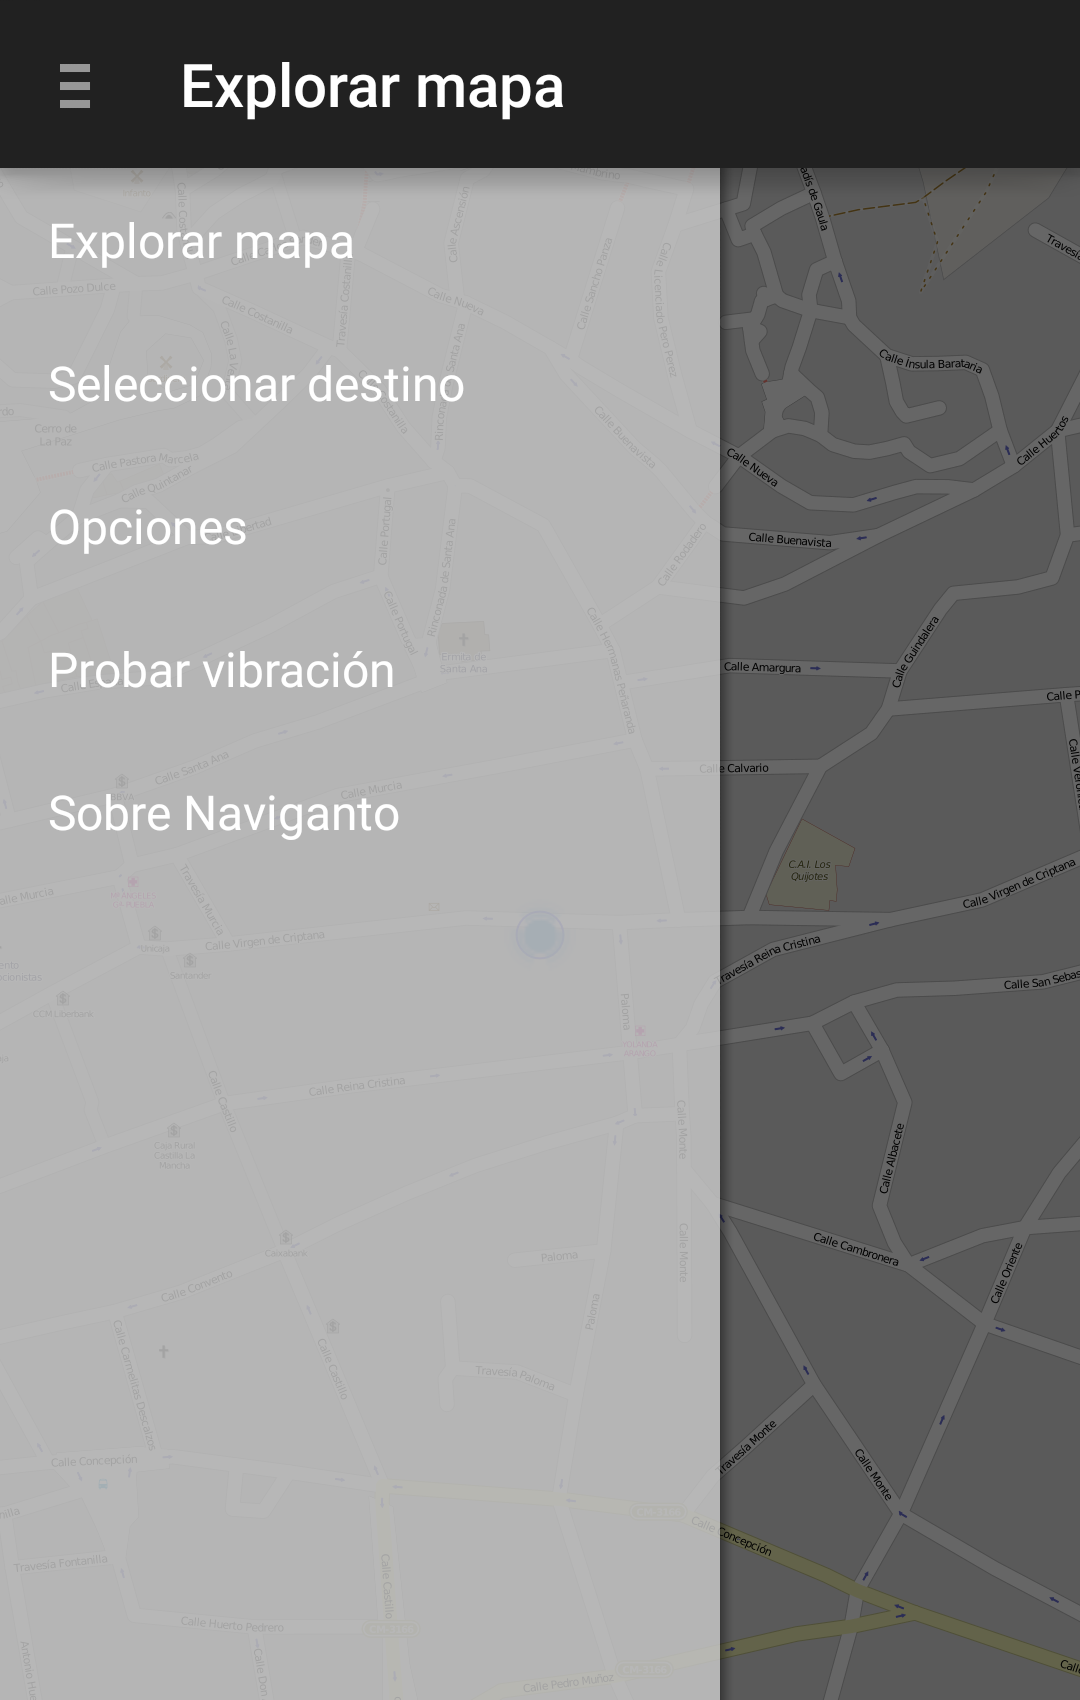
\includegraphics[width=0.85\textwidth]{/naviganto-barralateral.png}
    \end{center}
  \end{minipage}
  \begin{minipage}[b]{0.5\linewidth}
    \begin{center}
      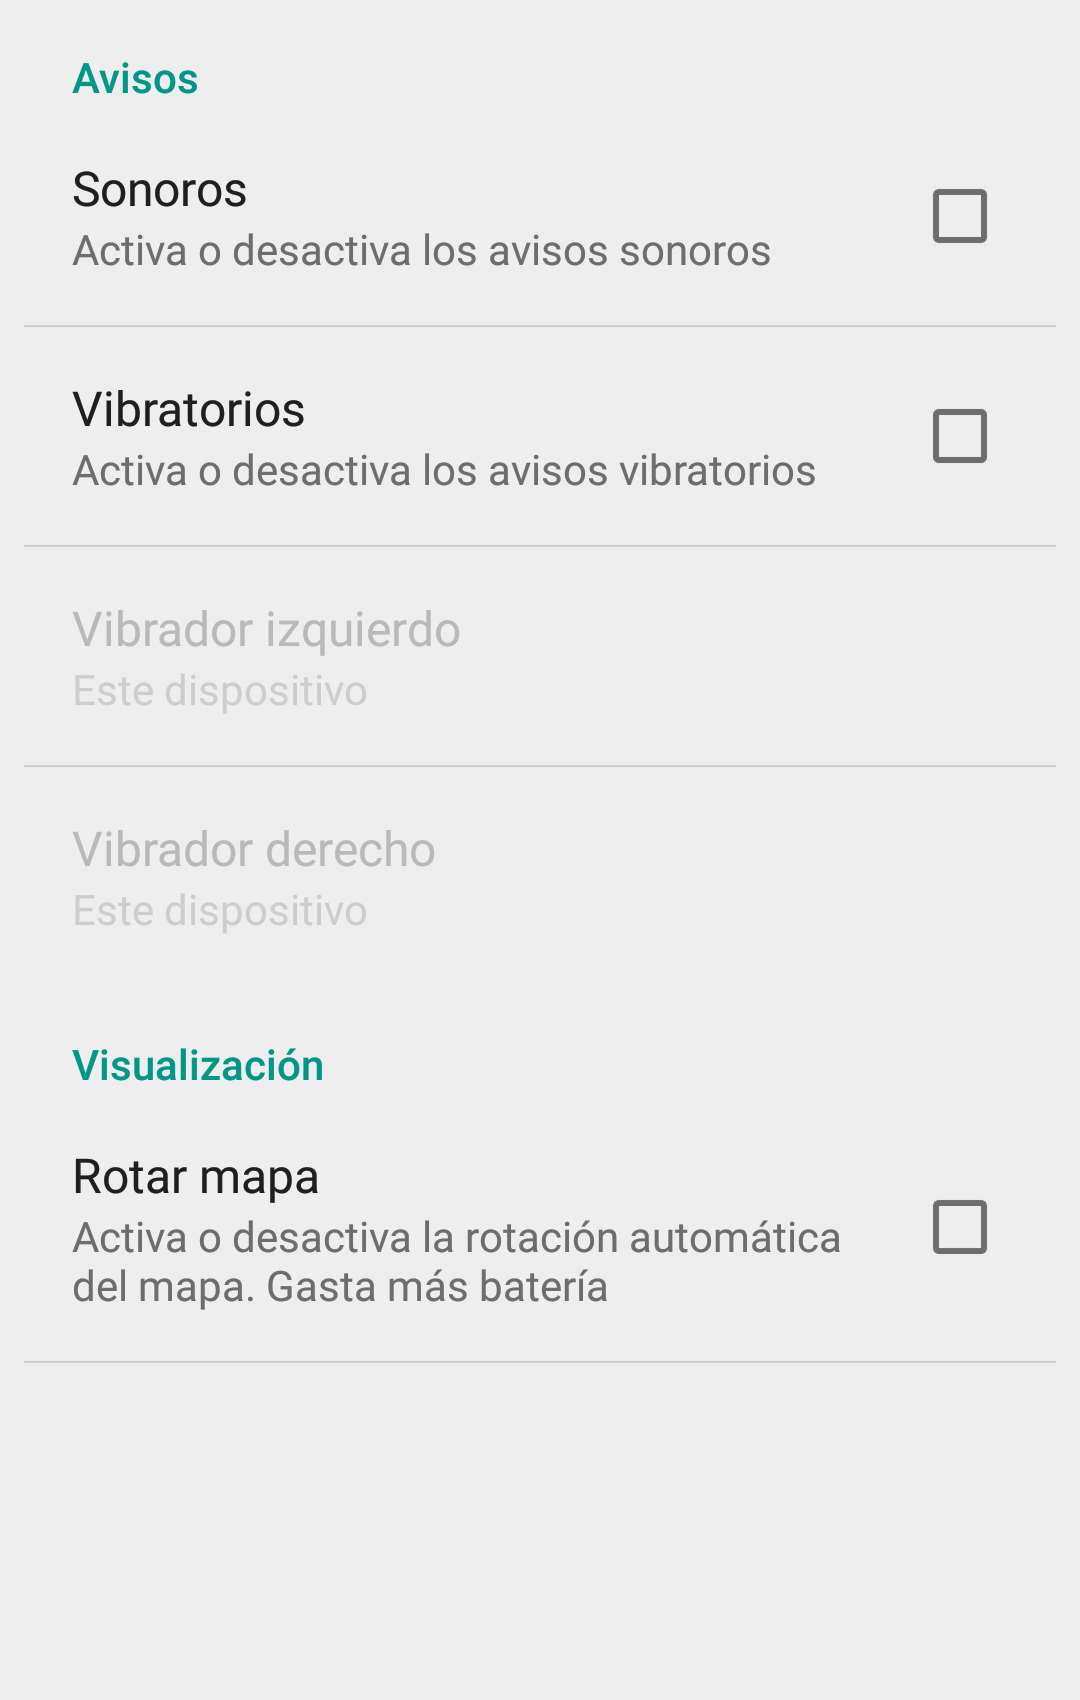
\includegraphics[width=0.85\textwidth]{/naviganto-opciones.png}
    \end{center}
  \end{minipage}
\end{figure}

Aquí podrá configurar las opciones descritas en los siguientes apartados.

\subsubsection{Avisos sonoros}
\subsubsection{Avisos vibratorios}
\subsubsection{Rotación de mapa}
\subsection{Navegación}
\subsubsection{Explorar mapa}
\subsubsection{Guiado por ruta}

% Local Variables:
% TeX-master: "main.tex"
%  coding: utf-8
%  mode: latex
%  mode: flyspell
%  ispell-local-dictionary: "castellano8"
% End:
